%%%%%%%%%%%%%%%%%%%%%%%%%%%%%%%%%%%%%%%%%%%%%%%%%%%%%%%%%%%%%%%%%%%%%%%%%%%%%%%%
%2345678901234567890123456789012345678901234567890123456789012345678901234567890
%        1         2         3         4         5         6         7         8

\documentclass[letterpaper, 10 pt, conference]{ieeeconf}
\makeatletter
\def\endthebibliography{%
  \def\@noitemerr{\@latex@warning{Empty `thebibliography' environment}}%
  \endlist
}
                                                          % if you need a4paper
%\documentclass[a4paper, 10pt, conference]{ieeeconf}      % Use this line for a4
                                                          % paper

\IEEEoverridecommandlockouts                              % This command is only
                                                          % needed if you want to
                                                          % use the \thanks command
\overrideIEEEmargins
% See the \addtolength command later in the file to balance the column lengths
% on the last page of the document



% The following packages can be found on http:\\www.ctan.org
%\usepackage{graphics} % for pdf, bitmapped graphics files
%\usepackage{epsfig} % for postscript graphics files
%\usepackage{mathptmx} % assumes new font selection scheme installed
%\usepackage{times} % assumes new font selection scheme installed
\usepackage{amsmath} % assumes amsmath package installed
\usepackage{amssymb}  % assumes amsmath package installed
\usepackage{boldline}
\usepackage{array,multirow}
\usepackage{dblfloatfix} 
\usepackage{hyperref}
\usepackage{float}
\usepackage{color}
\usepackage{xfrac}
\usepackage{graphicx}
\graphicspath{ {images/} }
\definecolor{light-gray}{gray}{0.95}
\newcommand{\code}[1]{\colorbox{light-gray}{\texttt{#1}}}
\DeclareMathOperator*{\argmax}{arg\,max}
\DeclareMathOperator*{\maxU}{max}
\usepackage{makecell}
\usepackage{bbm}
\usepackage[table,xcdraw]{xcolor}
\usepackage[flushleft]{threeparttable}
\usepackage[utf8]{inputenc}
\usepackage{capt-of}
\hypersetup{
    colorlinks=true,
    linkcolor=blue,
    filecolor=magenta,      
    urlcolor=cyan,
}


\usepackage{filecontents}

\begin{filecontents}{\jobname.bib}
@article{vinyals,
  author    = {Oriol Vinyals and
               Alexander Toshev and
               Samy Bengio and
               Dumitru Erhan},
  title     = {Show and Tell: {A} Neural Image Caption Generator},
  journal   = {CoRR},
  volume    = {abs/1411.4555},
  year      = {2014},
  url       = {http://arxiv.org/abs/1411.4555},
  archivePrefix = {arXiv},
  eprint    = {1411.4555},
  timestamp = {Wed, 07 Jun 2017 14:41:10 +0200},
  biburl    = {https://dblp.org/rec/bib/journals/corr/VinyalsTBE14},
  bibsource = {dblp computer science bibliography, https://dblp.org}
}

@article{kumar,
  author    = {Rajat Kumar Sinha and
               Ruchi Pandey and
               Rohan Pattnaik},
  title     = {Deep Learning For Computer Vision Tasks: {A} review},
  journal   = {CoRR},
  volume    = {abs/1804.03928},
  year      = {2018},
  url       = {http://arxiv.org/abs/1804.03928},
  archivePrefix = {arXiv},
  eprint    = {1804.03928},
  timestamp = {Tue, 01 May 2018 19:46:29 +0200},
  biburl    = {https://dblp.org/rec/bib/journals/corr/abs-1804-03928},
  bibsource = {dblp computer science bibliography, https://dblp.org}
}

@article{cho,
  author    = {Kyunghyun Cho and
               Bart van Merrienboer and
               {\c{C}}aglar G{\"{u}}l{\c{c}}ehre and
               Fethi Bougares and
               Holger Schwenk and
               Yoshua Bengio},
  title     = {Learning Phrase Representations using {RNN} Encoder-Decoder for Statistical
               Machine Translation},
  journal   = {CoRR},
  volume    = {abs/1406.1078},
  year      = {2014},
  url       = {http://arxiv.org/abs/1406.1078},
  archivePrefix = {arXiv},
  eprint    = {1406.1078},
  timestamp = {Wed, 07 Jun 2017 14:43:08 +0200},
  biburl    = {https://dblp.org/rec/bib/journals/corr/ChoMGBSB14},
  bibsource = {dblp computer science bibliography, https://dblp.org}
}



@article{tanti1,
  author    = {Marc Tanti and
               Albert Gatt and
               Kenneth P. Camilleri},
  title     = {Where to put the Image in an Image Caption Generator},
  journal   = {CoRR},
  volume    = {abs/1703.09137},
  year      = {2017},
  url       = {http://arxiv.org/abs/1703.09137},
  archivePrefix = {arXiv},
  eprint    = {1703.09137},
  timestamp = {Wed, 07 Jun 2017 14:43:03 +0200},
  biburl    = {https://dblp.org/rec/bib/journals/corr/TantiGC17},
  bibsource = {dblp computer science bibliography, https://dblp.org}
}

@article{tanti2,
  author    = {Marc Tanti and
               Albert Gatt and
               Kenneth P. Camilleri},
  title     = {What is the Role of Recurrent Neural Networks (RNNs) in an Image Caption
               Generator?},
  journal   = {CoRR},
  volume    = {abs/1708.02043},
  year      = {2017},
  url       = {http://arxiv.org/abs/1708.02043},
  archivePrefix = {arXiv},
  eprint    = {1708.02043},
  timestamp = {Tue, 05 Sep 2017 10:03:46 +0200},
  biburl    = {https://dblp.org/rec/bib/journals/corr/abs-1708-02043},
  bibsource = {dblp computer science bibliography, https://dblp.org}
}

@article{xu,
  author    = {Kelvin Xu and
               Jimmy Ba and
               Ryan Kiros and
               Kyunghyun Cho and
               Aaron C. Courville and
               Ruslan Salakhutdinov and
               Richard S. Zemel and
               Yoshua Bengio},
  title     = {Show, Attend and Tell: Neural Image Caption Generation with Visual
               Attention},
  journal   = {CoRR},
  volume    = {abs/1502.03044},
  year      = {2015},
  url       = {http://arxiv.org/abs/1502.03044},
  archivePrefix = {arXiv},
  eprint    = {1502.03044},
  timestamp = {Wed, 07 Jun 2017 14:43:05 +0200},
  biburl    = {https://dblp.org/rec/bib/journals/corr/XuBKCCSZB15},
  bibsource = {dblp computer science bibliography, https://dblp.org}
}
@inproceedings{8k,
 author = {Rashtchian, Cyrus and Young, Peter and Hodosh, Micah and Hockenmaier, Julia},
 title = {Collecting Image Annotations Using Amazon's Mechanical Turk},
 booktitle = {Proceedings of the NAACL HLT 2010 Workshop on Creating Speech and Language Data with Amazon's Mechanical Turk},
 series = {CSLDAMT '10},
 year = {2010},
 location = {Los Angeles, California},
 pages = {139--147},
 numpages = {9},
 url = {http://dl.acm.org/citation.cfm?id=1866696.1866717},
 acmid = {1866717},
 publisher = {Association for Computational Linguistics},
 address = {Stroudsburg, PA, USA},
}

@article{30k,
	author = {Young, Peter  and Lai, Alice  and Hodosh, Micah  and Hockenmaier, Julia },
	title = {From image descriptions to visual denotations: New similarity metrics for semantic inference over event descriptions},
	journal = {Transactions of the Association for Computational Linguistics},
	volume = {2},
	year = {2014},
	keywords = {},
	abstract = {We propose to use the visual denotations of linguistic expressions (i.e. the set of images they describe) to define novel denotational similarity metrics, which we show to be at least as beneficial as distributional similarities for two tasks that require semantic inference. To compute these denotational similarities, we construct a denotation graph, i.e. a subsumption hierarchy over constituents and their denotations, based on a large corpus of 30K images and 150K descriptive captions.},
	issn = {2307-387X},
	url = {https://transacl.org/ojs/index.php/tacl/article/view/229},
	pages = {67--78}
}
@article{coco,
  author    = {Tsung{-}Yi Lin and
               Michael Maire and
               Serge J. Belongie and
               Lubomir D. Bourdev and
               Ross B. Girshick and
               James Hays and
               Pietro Perona and
               Deva Ramanan and
               Piotr Doll{\'{a}}r and
               C. Lawrence Zitnick},
  title     = {Microsoft {COCO:} Common Objects in Context},
  journal   = {CoRR},
  volume    = {abs/1405.0312},
  year      = {2014},
  url       = {http://arxiv.org/abs/1405.0312},
  archivePrefix = {arXiv},
  eprint    = {1405.0312},
  timestamp = {Wed, 07 Jun 2017 14:41:35 +0200},
  biburl    = {https://dblp.org/rec/bib/journals/corr/LinMBHPRDZ14},
  bibsource = {dblp computer science bibliography, https://dblp.org}
}
\end{filecontents}


\title{\LARGE \bf
Everything Looks Like Chicken (and Waffles)
}

\author{ \large A Neural Image Captioning System, built on Yelp image data. A submission to the  \href{https://www.yelp.com/dataset/challenge}{Yelp Dataset Challenge.} \\ \\
	\parbox{2 in}{\centering Tamir Bennatan
         {\tt\small timibennatan@gmail.com}
}}

\begin{document}

\nocite{vinyals}
\nocite{tanti1}
\nocite{tanti2}
\nocite{cho}
\nocite{kumar}
\nocite{xu}
\nocite{8k}
\nocite{30k}
\nocite{coco}

\maketitle
\thispagestyle{empty}
\pagestyle{empty}

\begin{abstract}
This is filler. Here goes the abstract.This is filler. Here goes the abstract.This is filler. Here goes the abstract.This is filler. Here goes the abstract.This is filler. Here goes the abstract.This is filler. Here goes the abstract.This is filler. Here goes the abstract.This is filler. Here goes the abstract.This is filler. Here goes the abstract.This is filler. Here goes the abstract.This is filler. Here goes the abstract.This is filler. Here goes the abstract.This is filler. Here goes the abstract.This is filler. Here goes the abstract.This is filler. Here goes the abstract.This is filler. Here goes the abstract.This is filler. Here goes the abstract.
\end{abstract}


%%%%%%%%%%%%%%%%%%%%%%%%%%%%%%%%%%%%%%%%%%%%%%%%%%%%%%%%%%%%%%%%%%%%%%%%%%%%%%%%


%%%%%%%%%%%%%%%%%%%%%%%%%%%%%%%%%%%%%%%%%%%%%%%%%%%%%%%%%%%%%%%%%%%%%%%%%%%%%%%%
\section{INTRODUCTION}

Here is an introduction. I will detail what an NIC system is, why it's hard and useful. I talk about how other researchers use specialized datasets for image captioning, and how in this work I used a real life dataset, where the annotaters are not given any instructions. I then talk about the work that I did, briefly outline experiements, results, and mention that I do qualitative error checking. 

Here is an introduction. I will detail what an NIC system is, why it's hard and useful. I talk about how other researchers use specialized datasets for image captioning, and how in this work I used a real life dataset, where the annotaters are not given any instructions. I then talk about the work that I did, briefly outline experiements, results, and mention that I do qualitative error checking. 

Here is an introduction. I will detail what an NIC system is, why it's hard and useful. I talk about how other researchers use specialized datasets for image captioning, and how in this work I used a real life dataset, where the annotaters are not given any instructions. I then talk about the work that I did, briefly outline experiements, results, and mention that I do qualitative error checking. 

Here is an introduction. I will detail what an NIC system is, why it's hard and useful. I talk about how other researchers use specialized datasets for image captioning, and how in this work I used a real life dataset, where the annotaters are not given any instructions. I then talk about the work that I did, briefly outline experiements, results, and mention that I do qualitative error checking. 

\section{RELATED WORK}

In recent years, the deep learning community has have achieved great success in core computer vision tasks, such as image classification, object identification, and image extraction (Sinha et al. 2018). These successes, coupled with advancements in neural machine translation and language modeling technologies, have enabled researchers to develop end-to-end neural network models that can be used for image captioning systems. 

Vinyals et al (2014). describe such a system, which utilizes the power of Convolutional Neural Networks (CNN) for extracting complex visual features from images, and Recurrent Neural Networks (RNN) for generating new sequences. Inspired by the encoder-decoder framework for machine translation, the authors use a deep CNN to encode images to fixed-length vector representation, and feed this representation to an RNN which is used to generate a caption (further details in section III). 


\begin{figure*}[ht]
\centering
\begin{minipage}{.5\textwidth}
  \centering
  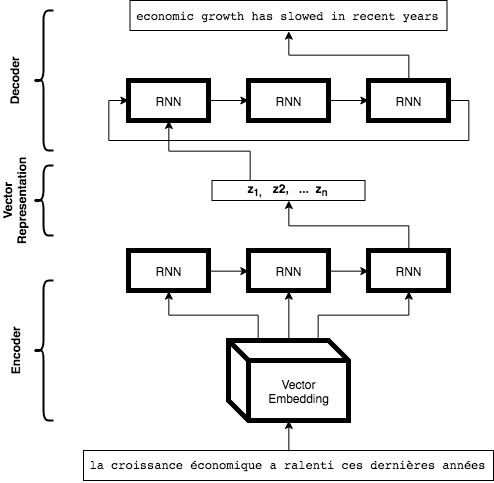
\includegraphics[width=.65\linewidth]{encoder_decoder_trans}
  \label{fig:test1}
\end{minipage}%
\begin{minipage}{.5\textwidth}
  \centering
  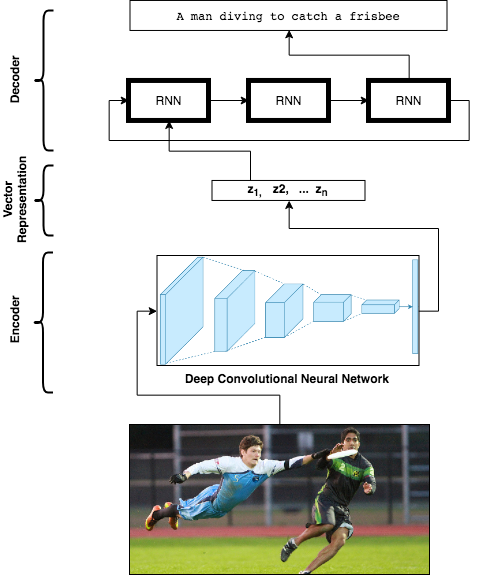
\includegraphics[width=.65\linewidth]{encoder_decoder_cnn}
  \label{fig:test2}
\end{minipage}
\caption{The encoder-decoder framework in neural machine translation models (left) and image captioning models (right). In machine translation applications, an input sequence is encoded by an RNN to a vector represention, before decoded to an output sequence. Analogously, a neural image captioning system uses a CNN to encode an input image before generating an output sequence.}
\end{figure*}

In their 2017 papers, Tanti et al. describe a set of architectures that fall under the general encoder-decoder framework. The primary difference between these architectures concerns how to feed the image features to the RNN layers, if at all. Tanti et al. rigorously test the efficacy of image captioning models with varying architectures on canonical image captioning datasets, in an attempt to deduce favorable architectures for image captioning models, and to form a conjecture as to what broad classes of tasks RNNs are best suited for.

Xu et al. (2016) achieve state of the art performance on standard datasets by incorporating an attention machanism. The authors argue that attention proves useful for the image captioning problem, as a network can learn to focus on the important features of an image, and ignore noisy features that result from cluttered images. Attention also provides additional interpretability to an image captioning model, as one can visualize what section of an image the attention is focused on at each time step. 

Previous work focuses on the use of specialized datasets that were collected for the purpose of image captioning and object segmentation tasks, such as Flickr-8k (Rashtchian et al.; 2010), Flickr-30k (Young et al.; 2014), and MS-COCO (Lin et al.; 2014). These datasets were collected by giving human annotators detailed instructions on how to annotate each image, resulting in relativly clean, albeit synthetic datasets. This work uses a much more difficult, real-world dataset collected by Yelp. As users are given no instructions on how to annotate each image before uploading it to the site, this dataset makes it much more difficult to learn an effective image captioning network. In this work, I discuss some of these difficulties, and undesireable behaviors that arise when training an image captioning network on such data. I also experiment with several architectures proposed by Tanti et al., in an attempt to study which architectures perform best under such circumstances.


\section{THEORETICAL BACKGROUND}

In this section, I discuss several abstract perspectives regarding the problem of Neural Image Captioning (NIC) which motivated many of the design choices and experiments that follow. First, I discuss how one can fit the problem of generating a caption of an image into the probablistic framework. Then, I briefly describe encoder-decoder models, and the NIC models I built are inspired by their encoder-decoder models in neural machine translation. Finally, I highlight an important design choice choosing the architecture of an NIC system, and the conceptual implication of this choice. 

\subsection{Training as Maximizing Caption Likelihood}

Although much of the work on image and video captioning involves stiching together several independent systems, researchers are achieving increasing success building individual neural networks that are fully trainable by back-propogation. Learning the parameters of such models has a natural probablistic interpretation; the objective is to directly maximize (with respect to the model weights, $\theta$) the probability of the correct caption given the weights and an image, $I$. For a dataset of $N$ image/caption pairs, this can be modeled as\footnote{Under the assumption that the correct captions the images are mutually independent.}:

\begin{equation}
\theta^* = \argmax_{\theta}{\sum_{i = 1}^N{\log(P(S^{(i)}|I^{(i)}; \theta)}}
\end{equation} 

Where $(S^{(i)}, I^{(i)})$ is the $i^{\text{th}}$ caption/image pair, and each caption $S^{(i)}$ is a sequence of tokens $(S^{(i)}_1, S^{(i)}_1, ... S^{(i)}_k)$ for a fixed maximum sequence length, $k$. 

We may simplify this by the chain rule of probability:

\begin{equation}
\theta^* = \argmax_{\theta}{\sum_{i = 1}^N{\sum_{t = 1}^k{P(S_t^{(i)}|S_{t - 1}^{(i)} ... S_{1}^{(i)}; \theta)}}}
\end{equation} 

Equation (2) is the inspiration for the training schema I used to learn the weights, to be discussed further in section \textbf{SECTION HERE}.

\section{METHODOLOGY}

We started by splitting the labeled data into training and validation splits of sizes 40,000 and 10,000 examples, respectively. We kept these splits consistent in all experiments, so that we could gauge the relative effectiveness our different models. For each of the three algorithms we used, we chose which size heuristic(s) to use based on which heuristic(s) yielded the highest validation accuracy when used to select the largest digit during preprocessing. We also used this validation set to tune model-specific parameters.

\subsection{Regularized Logistic Regression: Model Hyperparameters} 

The two hyperparamters we tuned the for logistic regression were the inverse-regularization coefficient, $C$\footnote{In the notation seen in class, $C \propto \sfrac{1}{\lambda}$.}, and the regularization loss function (either \emph{l1} or \emph{l2}). Using the processed datasets generated from using each of the four size heuristics, we ran a grid-search over 24 hyperparameter combinations, and selected the combination that yielded the best validation accuracy.   

\subsection{Feedforward Neural Network: Model Hyperparameters} 

The two hyperparameters we tuned when using FFNNs were the learning rate, $\eta$, and the model architecture. We did not implement regularization.

\subsection{Feedforward Neural Network: Learning Optimizations} 

We began by trying to fit our models using simple SGD, but quickly found that our models were not converging. 

To address this, we implemented \emph{momentum} to help calculate the ammount each weight $\theta$ should be updated on iteration $t$, denoted $\nu_t$, where $\nu_t$ is defined:
$$
\nu_t = \gamma\nu_{t-1} - \eta\nabla_{\theta}\text{Loss}(\theta)
$$
Where $\gamma$ is an additional hyperparameter introduced. 

We also implemented \emph{power scaling} - a method of slowly reducing the learning rate $\eta$ with each epoch. At the end of each epoch, $\eta$ is updated as follows:
$$
\eta_{\text{new}} = \frac{\eta_{\text{old}}}{(\text{Epoch number})^{p}}
$$
for a scaling parameter $p$. This allows the weights to change drastically in the begining of training, and slowly dampens the change in weights as training progresses, so that local maxima are not overlooked. 

We found that introducing these two learning optimizations helped the SGD algorithm minimize loss much faster. Thus, for all experiments with FFNN, we used both momentum and power scaling, with the hyperparameters fixed at $\gamma = .9, p = .9$. 

\subsection{Convolutional Neural Network: Hyperparameter Tuning} 

We considered many hyperparameters when tuning our CNN models. The most important hyperparameters are summarized in Table 1.
\begin{table}[b]
\caption{Hyperparameter Ranges Explored for CNN models}
\centering
\label{my-label}
\begin{tabular}{|c|c|}
\hline
\textbf{Hyperparameter}                                                                     & \textbf{Range Explored}                                                                                                            \\ \hline
Model Architecture                                                                          & \begin{tabular}[c]{@{}c@{}}\{Architecture 1, Architecture 2, \\ Architecture 3, Architecture 4\}\end{tabular}                      \\ \hline
\begin{tabular}[c]{@{}c@{}}Data Augmentation - \\ (Batch size, Rotation Range)\end{tabular} & \begin{tabular}[c]{@{}c@{}}\{(1, {[}0, 0{]}), \\ (8, {[}-10, 10{]}), \\ (16, {[}-20, 20{]}), \\ (16, {[}-30, 30{]})\}\end{tabular} \\ \hline
\multicolumn{1}{|l|}{Learning Rate}                                                         & \multicolumn{1}{l|}{\{.00001, .00005, .0001\}}                                                                                  \\ \hline
Digit Size Heuristic                                                                        & \begin{tabular}[c]{@{}c@{}}\{Heuristic 1, Heuristic 2,\\  Heuristic 3, Heuristic 4\}\end{tabular}                                  \\ \hline
\end{tabular}
\end{table}

We started by training all four architectures on the data preprocessed using Heuristic 1 with the high learning rate of $.0001$. After observing that architectures 2 and 4 yielded much higher validation accuracy than architectures 1 and 3, we decided to omit the latter architectures from all further experiments.

We then took a random sample of 64 images from EMNIST, and extracted the "largest" digit from each image using each of the four size heuristics defined. We observed by visual inspection that when using Heuristics 2 and 4, we isolated the digits corresponding to the labels more frequently than when we used Heuristics 1 and 3. We decided to use data preprocessed with Heuristics 2 and 4 in all further experiments. 

We then performed a gridsearch on the remaining hyperparameter combinations permitted by the constrained hyperparameter ranges [Table 2], totaling 32 hyperparamter combinations.


\begin{table}[]
\centering
\caption{Constrained Hyperparameter Ranges}
\label{my-label}
\begin{tabular}{|c|c|}
\hline
\textbf{Hyperparameter}                                                                     & \textbf{Range Explored}                                                                                                            \\ \hline
Model Architecture                                                                          & \{Architecture 2, Architecture 4\}                                                                                                 \\ \hline
\begin{tabular}[c]{@{}c@{}}Data Augmentation - \\ (Batch size, Rotation Range)\end{tabular} & \begin{tabular}[c]{@{}c@{}}\{(1, {[}0, 0{]}), \\ (8, {[}-10, 10{]}), \\ (16, {[}-20, 20{]}), \\ (16, {[}-30, 30{]})\}\end{tabular} \\ \hline
Learning Rate                                                                               & \{.00001, .00005\}                                                                                                               \\ \hline
Digit Size Heuristic                                                                        & \{Heuristic 2, Heuristic 4\}                                                                                                       \\ \hline
\end{tabular}
\end{table}


\subsection{CNN: Learning Optimization} 

We learned the weights of our networks using the \emph{RMSProp} algorithm, with the hyperparameter $\rho$ fixed at 0.9. While learning, we used an early stopping scheme, which caused training to stop if the validation accuracy has not improved for 8 consecutive epochs. 

At first, we tried learning using learning rate of $\eta = .0001$, but we observed through the use of learning curves that the convergence had very high variance. After reducing the learning rate to $.00005$, we achieved smoother learning [Figure 7]. Thus, we limited the range of values or $\eta$ to consider to $\eta \in \{.00005, .00001\}$.

\begin{figure}
      \centering
      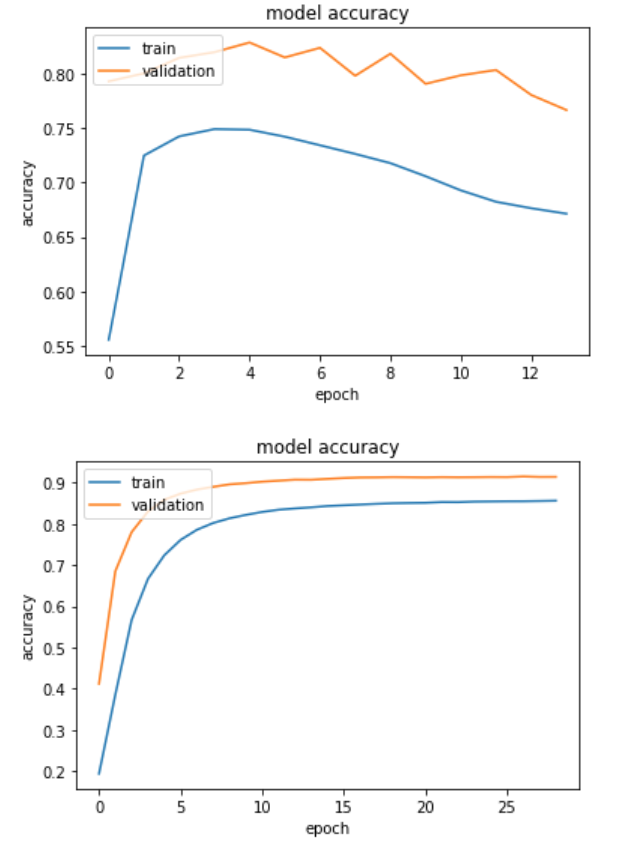
\includegraphics[scale = .6]{learning_curves.png}
		\centering
      %\includegraphics[scale=1.0]{figurefile}
      \caption{Learning curves for training periods with $\eta = .0001$ and $\eta = .00005$, with early stopping. Note: training accuracy is lower than validation accuracy. This is because we used data augmentation, and the new randomly rotated images made the training data "harder" to learn than the validation data.}
      \label{figurelabel}
\end{figure}

\subsection{CNN: Aggregated Predictions} 

We initialized the weights of our CNN's randomly. As such, every time we fit a CNN with fixed configuration, the final weights were not guaranteed to be the same, potentially leading to different predictions. 

To account for this randomness, we fit two models of each hyperparameter configuration, each with different random initialization. This allowed us to keep the better of the two trained models (based on validation-set accuracy) for each hyperparameter configuration. Further, this presented us with the opportunity to aggregate the predictions of our best performing CNN configurations\footnote{To aggregate predictions of several models, we used the class which was predicted the most frequently amongst all models to be the aggregated class prediction.}.

We experimented with the aggregations of the predictions of our four best CNN models, in terms of validation accuracy. We refer to these CNN configurations as \emph{CNN 1-4}. 

Two of these aggregations increased validation accuracy by over 1\%. We refer to these aggregations as \emph{Aggregation 1} and \emph{Aggregation 2}. 

\textbf{Aggregation 1:}
\begin{itemize}
\item Predictions of four models aggregated.
\item All four top CNN configurations used exactly once:
	\begin{itemize}
    \item CNN 1: Architechture 2, Batch Bize = 16, Rotation Range [-.2, .2], $\eta$ = .00005, Size Heuristic 2
	\item CNN 2: Architechture 4, Batch Bize = 16, Rotation Range [-.2, .2], $\eta$ = .00005, Size Heuristic 2
	\item CNN 3: Architechture 2, Batch Bize = 16, Rotation Range [-.2, .2], $\eta$ = .00005, Size Heuristic 4
	\item CNN 4: Architechture 4, Batch Bize = 16, Rotation Range [-.2, .2], $\eta$ = .00005, Size Heuristic 4
	\end{itemize}
\end{itemize}
\textbf{Aggregation 2:}
\begin{itemize}
\item Predictions of four models aggregated.
\item CNN 1 and CNN 2 were both trained twice with different intitializations, and included in the aggregation twice.
\end{itemize}

\section{RESULTS}

In this section we discuss the hyperparameters which had the largest impact on the performance of each model, and then we compare the perforance of each of our tuned models on the validation set. 

\subsection{Regularized Logistic Regression} 

After doing a thorough search through many $\big(\text{C}, \text{Regularization Loss Function}\big)$ combinations, we found that the hyperparameter which had the largest impact on validation accuracy was the regularization loss function. The best model trained with $l1$-loss achieved a validation accuracy over 1\% higher than the best model trained with $l2$-loss [Table 3].

\begin{table}[H]
\centering
\caption{Best Logistic Regression Models, Trained with l1/l2 Loss}
\label{my-}
\begin{tabular}{|c|c|c|}
\hline
\textbf{Loss Function} & \textbf{Regularization Parameter} & \textbf{Validation Accuracy} \\ \hline
l1-loss                & 0.09                              & 0.731                        \\ \hline
l1-loss                & .27                               & \textbf{0.735}               \\ \hline
l2-loss                & .01                               & 0.723                        \\ \hline
l2-loss                & .03                               & 0.721                        \\ \hline
\end{tabular}
\end{table}

Models trained with $l1$-loss regularization find sparse solutions - meaning that many input features do not contribute to the decision boundary. This has an interesting interpretation for the EMNIST classification problem; it means that the Logistic Regression model learned that some pixel values (features) do not help to predict the largest digit, and should be ignored.

For example, since we padded all images with a black border during preprocessing, these pixel values do not help to distinguish between the digits. Its reasonable to assume that the Logistic Regression model, trained with $l1$-loss learned to ignore the values of those pixels.

\subsection{Feedforward Neural Network} 

We experimented with three model architectures when fitting our FFNN:

\begin{table}[H]
\centering
\caption{FFNN Architectures}
\label{my-label}
\begin{tabular}{|c|c|c|}
\hline
\textbf{\begin{tabular}[c]{@{}c@{}}Architecture\\ Number\end{tabular}} & \textbf{\begin{tabular}[c]{@{}c@{}}Number of\\ Hidden Layers\end{tabular}} & \textbf{\begin{tabular}[c]{@{}c@{}}Hidden Layer\\ Dimensions\end{tabular}} \\ \hline
Architecture 1                                                         & 1                                                                          & (128)                                                                      \\ \hline
Architecture 2                                                         & 2                                                                          & (64, 20)                                                                   \\ \hline
Architecture 3                                                         & 2                                                                          & (128, 64)                                                                  \\ \hline
\end{tabular}
\end{table}

We trained all models for 20 epochs with SGD, using both momentum and power scaling. 

After some experimentations, we found that the configuration $\eta = .01, \gamma = .9, p = .9$ led to a reasonable convergence rate. Using these hyperparameter configurations, we fit each of the architectures described in table 3, and got the following results:

\begin{table}[H]
\centering
\caption{Validation Accuracies for FFNN Experiments}
\label{my-label}
\begin{tabular}{|c|c|}
\hline
\textbf{\begin{tabular}[c]{@{}c@{}}Architecture\\ Number\end{tabular}} & \textbf{\begin{tabular}[c]{@{}c@{}}Validation \\ Accuracy\end{tabular}} \\ \hline
Architecture 1                                                         & .55                                                                     \\ \hline
Architecture 2                                                         & .64                                                                     \\ \hline
Architecture 3                                                         & .64                                                                     \\ \hline
\end{tabular}
\end{table}

Of the three architectures we used, those with two hidden layers achieved almost 10\% better accuracy on the validation set. We have not tuned these models thoroughly, however, and so we cannot yet conclude that FFNNs with two hidden layers perform better on the EMNIST classification task than those with one hidden layer. Perhaps with more training, changes to the number of hidden units, and tuning to the learning hyperparameters $\gamma$ and $p$, a FFNN with one hidden unit could outperform Architectures 2 and 3. 

\subsection{Convolutional Neural Network} 

When training our CNNs, the performance of our models was not very sensitive to the learning rate $\eta$. In fact, we saw no evidence that models trained with the learning rate $\eta = .00001$ yielded higher validation accuracy than models trained with $\eta = .00005$ - all else fixed. 

A hyperparameter which had a noticeable effect was the choice of data augmentation scheme. Our best model trained without data augmentation yielded validation accuracy almost 2\% lower than our best model trained with data augmentation. 

We found that the benefits of data augmentation diminished as we increased the rotation range past $[-20,20]$. One explanation for this is that if one distorts the training data too severely, it makes the learning problem \emph{"too hard"}, and a classifier has trouble picking up on patterns in the modified training data. 

Thus, we found that the best configuration for data augmentation was a Batch Size of 16, with rotation range $[-20,20]$ [table 6].

% Please add the following required packages to your document preamble:
% \usepackage[table,xcdraw]{xcolor}
% If you use beamer only pass "xcolor=table" option, i.e. \documentclass[xcolor=table]{beamer}
\begin{table}[]
\centering
\caption{Best CNN Models for Different Data Augmentation Schemes}
\label{my-label}
\begin{tabular}{|c|c|
>{\columncolor[HTML]{ECF4FF}}c |
>{\columncolor[HTML]{ECF4FF}}c |
>{\columncolor[HTML]{ECF4FF}}c |}
\hline
\textbf{\begin{tabular}[c]{@{}c@{}}CNN\\ Architecture\end{tabular}} & \textbf{\begin{tabular}[c]{@{}c@{}}Digit Size\\ Heuristic\end{tabular}} & \textbf{\begin{tabular}[c]{@{}c@{}}Batch\\ Size\end{tabular}} & \textbf{\begin{tabular}[c]{@{}c@{}}Rotation\\ Range\end{tabular}} & \textbf{\begin{tabular}[c]{@{}c@{}}Validation\\ Accuracy\end{tabular}} \\ \hline
4                                                                   & 2                                                                       & 1                                                             & -                                                                 & 89.4                                                                   \\ \hline
4                                                                   & 2                                                                       & 16                                                            & {[}-20, 20{]}                                                     & \textbf{91.2}                                                          \\ \hline
4                                                                   & 2                                                                       & 16                                                            & {[}-30, 30{]}                                                     & 90.3                                                                   \\ \hline
\end{tabular}
\end{table}

We also found that aggregating predictions of serveral models led to an increase in validation accuracy.

The four CNN configurations which achieved the best validation accuracy are specified in section \emph{4.f}, and are referred to as \emph{CNN 1-4}. The predictions of these models were pooled to create Aggregation 1. The pooled predictions of Aggregation 1 achieved better validation accuracy than any of the individual models used to construct it. Further, we found that Aggregation 2 yielded the best validation accuracy [Table 7]. 

\begin{table}[b]
\centering
\caption{Highest performing CNN Models and Aggregations}
\label{my-label}
\begin{tabular}{|c|c|}
\hline
\textbf{\begin{tabular}[c]{@{}c@{}}CNN \\ Configuration\end{tabular}} & \textbf{\begin{tabular}[c]{@{}c@{}}Validation \\ Accuracy\end{tabular}} \\ \hline
CNN 1                                                                 & .910                                                                    \\ \hline
CNN 2                                                                 & .918                                                                    \\ \hline
CNN 3                                                                 & .906                                                                    \\ \hline
CNN 4                                                                 & .911                                                                    \\ \hline
\end{tabular}
\begin{tabular}{|l|l|}
\hline
\textbf{Aggregation} & \textbf{\begin{tabular}[c]{@{}l@{}}Validation \\ Accuracy\end{tabular}} \\ \hline
Aggregation 1        & .921                                                                    \\ \hline
Aggregation 2        & \textit{\textbf{.929}}                                                  \\ \hline
\end{tabular}
Validation accuracies of best four CNN configurations, and those of aggregated predictions. Aggregation 1 was created by pooling the predicions of CNN 1-4 once, and Aggregation 2 was created by pooling the predictions of CNN 1 and 2 twice - after training both configurations twice with different initializations.
\end{table}

This may suggest that the errors which of each of the models that we pooled "canceled out," simulating the predictions of a classifier with lower variance and increased prediction performance. Furthermore, due to the fact that all four models used to construct Aggregation 2 were trained on data preprocessed using Size Heuristic 2 - and that the predictions of Aggregation 2 led to the highest validation accuracy we achieved - we are inclined to believe that Heuristic 2 does the best job of identifying the "largest" digit in each image amongst the heuristics we proposed. 

Overall, our CNN models had the performed the best out of all our models; our final predictions were those of Aggregation 2 - with a validation accuracy of 92.9\% and a public leaderboard accuracy of 93.0\%. This validates our initial hypothesis that CNNs are an appropriate model class for the EMNIST classification problem.

\section{DISCUSSION AND CONCLUSIONS}

After running our experiments, we have concluded that CNNs achieve the best performance out of the three model classes that we trained. However, due to performance issues, we did not tune the hyperparameters of our FFNNs thoroughly enough to conclude that FFNN cannot achieve competitive performance. We would likely benefit from tuning our model architectures, and allowing our networks to train for more epochs. 

Furthermore our FFNN implmentation was very simplistic. Some of the optimizations we could implement that would likely help performance are:

\begin{itemize}
\item Regularization, and tune regularization parameter. We could also try to limit overfitting by implementing dropout.
\item Experiment with more learning methods (besides SGD), such as Batch Gradient Descent, and more advanced update rules, such as RMSProp or ADAM.
\item Backpropogation optimizations, such as Batch Normalization.  
\end{itemize}

Although we meticulously tuned the hyperparameters associated with our CNN models, we only considered a limited scope of model architectures. All four architectures we experimented with were variants of the LeNet architecture. 

Although LeNet has proved effective in classifying handwritten digits by many authors, we would like to experiment with a more diverse range of architectures in the future. One particularly exciting recent development in deep learning are Capsule Networks, proposed by Hinton et al. (2017), which may be more robust to changes in image orientation and overlapping images than CNNs - and thus applicable to this problem. 

Finally, we would like to invest more effort in improving our preprocessing methods. After visual inspection of 100 misclassified validation examples, we noticed that many of the digits that we extracted from these examples did not correspond to the correct label - meaning that we failed to extract the "largest" digit during preprocessing. We believe that our preprocessing is the bottleneck hindering us from building a more successful classifier, and that if we were to improve our preprocessing methods substantially then we could produce a more competitive solution. 



\bibliographystyle{IEEEtran}
\bibliography{\jobname}
\end{document}
